\documentclass[12pt, a4paper]{article}
\usepackage[pdftex]{graphicx} %for embedding images
\usepackage[utf8]{vietnam}
\usepackage{enumitem}
\usepackage[fleqn,tbtags]{amsmath}
\usepackage[ruled]{algorithm2e}
\usepackage{amsfonts}
\usepackage{amssymb}
\usepackage{tikz,tkz-tab}
\usetikzlibrary{matrix}
\usepackage{listings}
\usepackage{xcolor}
\usepackage[font=small,labelfont=bf]{caption}
\definecolor{codegreen}{rgb}{0.3,0.6,0.3}
\definecolor{codegray}{rgb}{0.5,0.5,0.5}
\definecolor{codepurple}{rgb}{0.58,0.1,0.82}
\lstset{
  language=C++, % choose the language of the code
  basicstyle=\ttfamily\small, % the size and style of the fonts that are used for the code
  keywordstyle=\color{blue}, % style for keywords
  stringstyle=\color{codepurple}, % style for strings
  commentstyle=\color{codegreen}, % style for comments
  showstringspaces=false,
  breaklines=true,
  backgroundcolor=\color{codegray!10}, % background color,
  numbers=left
}
%% This declares a command \Comment
%% The argument will be surrounded by /* ... */
\SetKwComment{Comment}{/* }{ */}
\SetKwProg{Fn}{Function}{}{}
\begin{document}

\pagenumbering{roman} %numbering before main content starts

\begin{titlepage}

\begin{center}


\includegraphics[width=1\textwidth]{img/banner_uit.png}\\%\\[0.1in]
\vspace{3em}%
% Title
\Large \textbf {BÀI TẬP MÔN\\PHÂN TÍCH VÀ
THIẾT KẾ THUẬT TOÁN}\\%\\[0.5in]
\vspace{1em}%
\normalsize by \\%
\vspace{1em}
\textup{\small {\bf Hoàng Quang Khải - 21520952}\\
{\bf Lê Tuấn Vũ - 21521679}\\
{\bf Nguyễn Nhật Minh - 21521135}\\
{\bf Lê Tiến Quyết - 21520428}\\}
 \vspace{1em}%
{\bf Faculty of Computer Science}\\[0.5in]

\emph{Homework \#01: Đánh giá thuật toán dùng kỹ thuật toán sơ cấp}

\vspace{1in}

    
% Submitted by
\normalsize {\bf GV hướng dẫn:} \\

Huỳnh Thị Thanh Thương\\
\vspace{1em}

\vfill

% Bottom of the page

TPHCM, March 9, 2023

\end{center}

\end{titlepage}


\newpage
\pagenumbering{arabic} %reset numbering to normal for the main content

\section{Tính tổng hữu hạn}
\begin{enumerate}[label=\alph*)]
    \item $\displaystyle 1+3+5+7+\ldots+999=\frac{n(2a_1+(n-1)d)}{2}=\frac{500\left(2+499.2\right)}{2}=250000$
    \item $\displaystyle 2+4+8+16+\ldots+1024=\frac{u_{1}(q^{n}-1)}{q-1}=\frac{2(2^{10}-1)}{2-1}=2046$
    \item $\displaystyle \sum_{i=3}^{n+1}1=n+1-3+1=n-1$
    \item $\displaystyle \sum_{i=3}^{n+1}i=\sum_{i=1}^{n+1}i-\sum_{i=1}^{2}i=\frac{(n+1)(n+2)}{2}-3=\frac{1}{2}\left(n^{2}+3n-4\right)
    $
    \item 
    \begin{multline*}
    \displaystyle \sum_{i=0}^{n-1}i(i+1)=\sum_{i=0}^{n-1}(i^{2}+i)=\sum_{i=0}^{n-1}i^{2}+\sum_{i=0}^{n-1}i\\=\frac{n(n-1)(2n-1)}{6}+\frac{n(n-1)}{2}=\frac{n(n+1)^{2}}{3}
    \end{multline*}
    \item
    \begin{multline*}
    \displaystyle\sum_{j=1}^{n}3^{j+1}=3\sum_{j=1}^{n}3^{j}=3\left(\sum_{j=0}^{n}3^{j}-3^{0}\right)=3\left(\frac{3^{n+1}-1}{3-1}-1\right)=\frac{3^{n+2}-9}{2}\\=\frac{9}{2}(3^{n}-1)
    \end{multline*}
    \item $\displaystyle
    \sum_{i=1}^{n}\sum_{j=1}^{n}ij=\sum_{i=1}^{n}i\frac{n(n+1)}{2}=\frac{n(n+1)}{2}\frac{n(n+1)}{2}=\frac{(n^{2}+n)^{2}}{4}
    $
    \item 
    \begin{multline*}
    \displaystyle
    \sum_{i=1}^{n}\frac{1}{i(i+1)}=\sum_{i=1}^{n}i\left(\frac{1}{i}-\frac{1}{i+1}\right)=\frac{1}{1}-\frac{1}{2}+\frac{1}{2}-\frac{1}{3}+\ldots+\frac{1}{n}-\frac{1}{n+1} \\=\frac{n}{n+1}
    \end{multline*}
    \item
    $\displaystyle\sum_{j\in\{2,3,5\}}(j^{2}+j)=(2^{2}+2)+(3^{2}+3)+(5^{2} +5)=48
    $
    \item
    \begin{multline*}
    \displaystyle
    \sum_{i=1}^{m}\sum_{j=0}^{n}\sum_{k=0}^{100}(i+j)=101\sum_{i=1}^{m}\sum_{j=0}^{n}(i+j)=101\sum_{i=1}^{m}\left[i(n+1)+\frac{n(n+1)}{2}\right]\\=101\left[\frac{m(n+1)(m+1)}{2}+\frac{mn(n+1)}{2}\right]=\frac{101}{2}m(n+1)(m+n+1)
    \end{multline*}
\end{enumerate}
\section{Đếm số phép gán và so sánh}
\begin{algorithm}[H]
    $s \gets 0$\Comment*[r]{2g}
    $i \gets 1$\;
    \While{$i\leq n$}{
    $j \gets1$\Comment*[r]{1g; n+1 ss}
    \While{$j\leq i^{2}$}{ 
    $s \gets s+1$ \Comment*[r]{2g}
    $j \gets j+1$\;
    }
    $i \gets i+1$\Comment*[r]{1g}
    }
\end{algorithm}
\vspace{1em}
Gọi $\alpha_{i}$ là số lần lặp của vòng lặp \textbf{while} nhỏ với điều kiện $j \leq i^{2} \quad(\alpha_{i} \geq 1)$ \\
Vì $\alpha_{i}$ là số con $j$ mà $j$ chạy từ 1 $\rightarrow i^{2}$ với bước tăng là 1. \\ 
Do đó, $\alpha_{i}$ nhận các giá trị $\{1, 4, 9,\ldots,i^{2}\} \rightarrow \alpha_{i} = i^{2}$
\vspace{1em}\\
\textbf{Kết luận}
\begin{flalign*}
\displaystyle 
\text{Gán}(n)&=2+2n+\sum_{i=1}^{n}2\alpha_{i}=2+2n+2\sum_{i=1}^{n}i^{2}=2+2n+\frac{n(n+1)(2n+1)}{3}\\&=\frac{2n^{3}+3n^{2}+7n+6}{3}
\end{flalign*}
\begin{flalign*}
\displaystyle
\text{Sosánh}(n)&=n+1+\sum_{i=1}^{n}(\alpha_{i}+1)=n+1+\sum_{i=1}^{n}i^{2}+\sum_{i=1}^{n}1\\&=2n+1+\frac{n(n+1)(2n+1)}{6}=\frac{2n^{3}+3n^{2}+13n+6}{6}
\end{flalign*} 
\section{Đếm số phép gán và so sánh}
\begin{algorithm}[H]
    $s \gets 0$\Comment*[r]{2g}
    $i \gets 1$\;
    \While{$i\leq n$}{
    $j \gets n-i^{2}$\Comment*[r]{1g; n+1 ss}
    \While{$j\leq i^{2}$}{ 
    $s \gets s+ij$ \Comment*[r]{2g}
    $j \gets j+1$\;
    }
    $i \gets i+1$\Comment*[r]{1g}
    }
\end{algorithm}
\vspace{1em}
Gọi $\alpha_{i}$ là số lần lặp của vòng lặp \textbf{while} nhỏ với điều kiện $j \leq i^{2} \quad(\alpha_{i} \geq 1)$ \\
Vì $\alpha_{i}$ là số con $j$ mà $j$ chạy từ $n-i^{2}$ $\rightarrow i^{2}$ với bước tăng là 1. \\ 
Do đó, $\alpha_{i}$ nhận các giá trị $\{n-i^{2},\ldots,i^{2}\}$\\
$\Rightarrow \alpha_{i} = i^{2}-(n-i^{2})+1=2i^{2}-n+1$\\
Với $\displaystyle\alpha_{i} \geq 1 \Leftrightarrow n-i^{2}-i^{2} \leq 0 \Rightarrow i \geq \left\lceil\sqrt{\frac{n}{2}}\right\rceil \quad(i \geq 1)$
\vspace{1em}\\
\textbf{Ta có:}
\begin{flalign*}
\displaystyle 
\text{Gán}(n)&=2+2n+\sum_{i=1}^{n}2\alpha_{i}=2+2n+2\sum_{i=1}^{n}(2i^{2}-n+1)\\&=2+2n+2\sum_{i=\left\lceil\sqrt{\frac{n}{2}}\right\rceil}^{n}(2i^{2}-n+1)
\end{flalign*}
\begin{flalign*}
\displaystyle
\text{Sosánh}(n)&=n+1+\sum_{i=1}^{n}(\alpha_{i}+1)=n+1+\sum_{i=1}^{n}\alpha_{i}+\sum_{i=1}^{n}1\\&=2n+1+\sum_{i=\left\lceil\sqrt{\frac{n}{2}}\right\rceil}^{n}(2i^{2}-n+1)
\end{flalign*}
Đặt $t=\left\lceil\sqrt{\frac{n}{2}}\right\rceil$, ta được:
\begin{multline*}
\displaystyle
    \sum_{i=\left\lceil\sqrt{\frac{n}{2}}\right\rceil}^{n}(2i^{2}-n+1)=\sum_{i=t}^{n}(2i^{2}-n+1)=\sum_{i=t}^{n}(-n+1)+2\sum_{i=t}^{n}i^{2}\\=(-n+1)(n-t+1)+2\sum_{i=1}^{n}i^{2}-2\sum_{i=1}^{t-1}i^{2}\\=(-n+1)(n-t+1)+\frac{n(n+1)(2n+1)}{3}-\frac{t(t-1)(2t-1)}{3}
\end{multline*}
\textbf{Kết luận}
\begin{flalign*}
    \text{Gán}(n)&=2+2n+2(-n+1)(n-t+1)+\frac{2}{3}[n(n+1)(2n+1)-t(t-1)(2t-1)]\\&=4+2(-n+1)(n-t)+\frac{2}{3}[n(n+1)(2n+1)-t(t-1)(2t-1)]
\end{flalign*}
\begin{flalign*}
    \text{Sosánh}(n)&=2n+1+(-n+1)(n-t+1)+\frac{1}{3}[n(n+1)(2n+1)-t(t-1)(2t-1)]\\&=2+n+(-n+1)(n-t)+\frac{1}{3}[n(n+1)(2n+1)-t(t-1)(2t-1)]
\end{flalign*}
Với $t=\left\lceil\sqrt{\frac{n}{2}}\right\rceil$

\section{Đếm số phép gán và so sánh}
\begin{algorithm}[H]
float \Fn {Alpha (float $x$, long $n$)}{
    long $i \gets 1$\Comment*[r]{2g}
    float $z\gets 0$\;
    \While{$i \leq n$}{
        long $j\gets 1$\Comment*[r]{2g; n+1 ss}
        float $t\gets 1$\;
        \While{$j\leq i$}{
            $t\gets tx$\Comment*[r]{2g}
            $j\gets 2j$\;
        }
        $z\gets z+it$\Comment*[r]{2g}
        $i\gets i+1$\;
    }
    return $z$\;
}
\end{algorithm}
Gọi $\alpha_{i}$ là số lần lặp của vòng lặp \textbf{while} nhỏ với điều kiện $j \leq i \quad(\alpha_{i} \geq 1)$\\
Vì $\alpha_{i}$ là số con $j$ mà $j$ chạy từ 1 $\rightarrow i$ với tỉ lệ bước tăng là 2.\\
Và $j$ nhận các giá trị $\{1,2,4,8,16,\ldots,2^{k}\}$, $k\in \mathbb{N}$\\
Do đó: $\alpha_{i} \text{ là số phần tử của tập } \{k\in\mathbb{N}\mid 2^{k}\leq i\} \Rightarrow 0 \leq k \leq \log_{2}i$\\
$\Rightarrow \alpha_{i} = \lfloor\log_{2}i\rfloor + 1$
\vspace{1em}\\
\textbf{Kết luận}
\begin{flalign*}
\displaystyle 
\text{Gán}(n)&=2+4n+\sum_{i=1}^{n}2\alpha_{i}=2+4n+2\sum_{i=1}^{n}(\lfloor\log_{2}i\rfloor + 1)\\&=2+4n+2\sum_{i=1}^{n}\lfloor\log_{2}i\rfloor+2\sum_{i=1}^{n}1=2+6n+2\sum_{i=1}^{n}\lfloor\log_{2}i\rfloor
\end{flalign*}
\begin{flalign*}
\displaystyle
\text{Sosánh}(n)&=n+1+\sum_{i=1}^{n}(\alpha_{i}+1)=n+1+\sum_{i=1}^{n}\lfloor\log_{2}i\rfloor+\sum_{i=1}^{n}2\\&=3n+1+\sum_{i=1}^{n}\lfloor\log_{2}i\rfloor
\end{flalign*}
\section{Đếm số phép gán và so sánh}
\begin{algorithm}[H]
    $sum \gets 0$\Comment*[r]{2g}
    $i \gets 1$\;
    \While{$i \leq n$}{
        $j \gets n - i$\Comment*[r]{1g; n+1 ss}
        \While{$j \leq 2i$}{
            $sum \gets sum+ij$\Comment*[r]{2g}
            $j\gets j+2$\;
        }
        $k\gets i$\Comment*[r]{1g}
        \While{$k > 0$}{
            $sum\gets sum+1$\Comment*[r]{2g}
            $k\gets k/2$\;
        }
        $i\gets i+1$\Comment*[r]{1g}
    }
\end{algorithm}
Gọi $\alpha_{i}$ là số lần lặp của vòng lặp \textbf{while} nhỏ với điều kiện $j \leq 2i$.\\
Vì $\alpha_{i}$ là số con $j$ mà $j$ chạy từ $n-i$ $\rightarrow 2i$ với bước tăng là 2.\\
Do đó: 
\begin{flalign*}
\displaystyle\alpha_{i} \text{ là số phần tử của tập } \{n-i,n-i+2,\ldots,2i\} &=\frac{2i-(n-i)}{2}+1\\&=\frac{3i-n+2}{2}
\end{flalign*}
$\displaystyle\text{Với }\alpha_{i} \geq 1 \Leftrightarrow n-i \leq 2i \Leftrightarrow i \geq \frac{n}{3}$.\\
Vậy:
\begin{flalign*}
\alpha_{i}=\left\{\begin{array}{l}
    \displaystyle0,\quad  i<\left\lceil\frac{n}{3} \right\rceil\vspace{1em}\\
    \displaystyle\frac{3i-n+2}{2}, \quad i \geq \left\lceil\frac{n}{3}\right\rceil
\end{array}\right.
\end{flalign*}
\vspace{1em}\\
\indent Gọi $\beta_{i}$ là số lần lặp của vòng lặp \textbf{while} nhỏ với điều kiện $k > 0$. \\
Vì $\beta_{i}$ là số con $j$ mà $j$ chạy từ $i$ $\rightarrow 1$ với tỉ lệ bước giảm là $\displaystyle\frac{1}{2}$.\\
Do đó:
\begin{flalign*}
    \beta_{i} \text{ là số phần tử của tập } \left\{i,\frac{i}{2},\frac{i}{4},\ldots,\frac{i}{2^{k}} \mid k\in \mathbb{N}, \frac{i}{2^{k}} \geq 1\right\}  \Rightarrow 0 \leq k\leq \left\lfloor\log_{2}i\right\rfloor  
\end{flalign*}
Vậy:
\begin{flalign*}
    \beta_{i} =\left\lfloor\log_{2}i\right\rfloor+1
\end{flalign*}
\textbf{Ta có}
\begin{flalign*}
\displaystyle 
\text{Gán}(n)&=2+3n+\sum_{i=1}^{n}2\alpha_{i}+\sum_{i=1}^{n}2\beta_{i}\\&=2+3n+\sum_{i=\left\lceil\frac{n}{3} \right\rceil}^{n}(3i-n+2)+2\sum_{i=1}^{n}(\lfloor\log_{2}i\rfloor+1)\\&=2+5n+\sum_{i=\left\lceil\frac{n}{3} \right\rceil}^{n}(3i-n+2)+2\sum_{i=1}^{n}\lfloor\log_{2}i\rfloor
\end{flalign*}
\begin{flalign*}
\displaystyle
\text{Sosánh}(n)&=n+1+\sum_{i=1}^{n}(\alpha_{i}+1)+\sum_{i=1}^{n}(\beta_{i}+1)\\&=n+1+\sum_{i=1}^{n}\alpha_{i}+\sum_{i=1}^{n}\beta_{i}+2\sum_{i=1}^{n}1\\&=3n+1+\frac{1}{2}\sum_{i=\left\lceil\frac{n}{3} \right\rceil}^{n}(3i-n+2)+\sum_{i=1}^{n}(\lfloor\log_{2}i\rfloor+1)\\&=4n+1+\frac{1}{2}\sum_{i=\left\lceil\frac{n}{3} \right\rceil}^{n}(3i-n+2)+\sum_{i=1}^{n}\lfloor\log_{2}i\rfloor
\end{flalign*}
Đặt $t=\left\lceil\frac{n}{3} \right\rceil$, ta được:\\
\begin{multline*}
    \sum_{i=\left\lceil\frac{n}{3} \right\rceil}^{n}(3i-n+2)=\sum_{i=t}^{n}(-n+2)+3\sum_{i=t}^{n}i\\=(-n+2)(n-t+1)+\frac{3}{2}(n-t+1)(n+t)
\end{multline*}
\textbf{Kết luận}
\begin{flalign*}
\displaystyle 
\text{Gán}(n)&=2+5n+(-n+2)(n-t+1)+\frac{3}{2}(n-t+1)(n+t)+2\sum_{i=1}^{n}\lfloor\log_{2}i\rfloor\\&=4+\frac{15}{2}n+\frac{1}{2}n^{2}+\frac{1}{2}t(2n-1)-\frac{3}{2}t^{2}+2\sum_{i=1}^{n}\lfloor\log_{2}i\rfloor
\end{flalign*}
\begin{flalign*}
\displaystyle
\text{Sosánh}(n)&=4n+1+\frac{1}{2}(-n+2)(n-t+1)+\frac{3}{4}(n-t+1)(n+t)+\sum_{i=1}^{n}\lfloor\log_{2}i\rfloor\\&=2+\frac{21}{4}n+\frac{1}{4}n^{2}+\frac{1}{4}t(2n-1)-\frac{3}{4}t^{2}+\sum_{i=1}^{n}\lfloor\log_{2}i\rfloor
\end{flalign*}
\section{Đếm số phép gán và so sánh} %Câu 6
\begin{algorithm}[H]
    $i\gets 1$\Comment*[r]{2g}
    $count\gets 0$\;
    \While{$i\leq 4n$}{
    $x\gets (n - i)(i - 3n)$\Comment*[r]{3g; 4n+1 ss}
    $y\gets i-2n$\;
    $j\gets 1$\;
    \While{$j \leq x$}{
        $count\gets count-2$\Comment*[r]{2g}
        $j\gets j+2$\;
    }
    \If{$x>0$}{
        \If{$y>0$}{
            $count\gets count + 1$\Comment*[r]{1g}
        }
    }
    $i\gets i+1$\Comment*[r]{1g}
    }
\end{algorithm}
Gọi $\alpha_{i}$ là số lần lặp của vòng lặp \textbf{while} nhỏ với điều kiện $j \leq x$.\\
Vì $\alpha_{i}$ là số con $j$ mà $j$ chạy từ 1 $\rightarrow x$ với bước tăng là 2.\\
Do đó: 
\begin{flalign*}
\displaystyle\alpha_{i} \text{ là số phần tử của tập } \{1,3,5,\ldots,x\} &=\frac{x-1}{2}+1=\frac{x+1}{2}\approx\left\lceil\frac{x}{2}\right\rceil\\&\approx\left\lceil\frac{(n-i)(i-3n)}{2}\right\rceil
\end{flalign*}
$\displaystyle\text{Với }\alpha_{i} \geq 1 \Leftrightarrow n+1 \leq i\leq 3n-1$.
\newpage
\vspace{1em}
Vậy:
\begin{gather*}
    \alpha_{i}=\left\{\begin{array}{l}
    \displaystyle0,\quad  i \leq n \text{ hoặc } i\geq 3n\vspace{1em}\\
    \displaystyle\left\lceil\frac{(n-i)(i-3n)}{2}\right\rceil, \quad n+1 \leq i\leq 3n-1
    \end{array}\right.
\end{gather*}
Ta có bảng xét dấu:\\
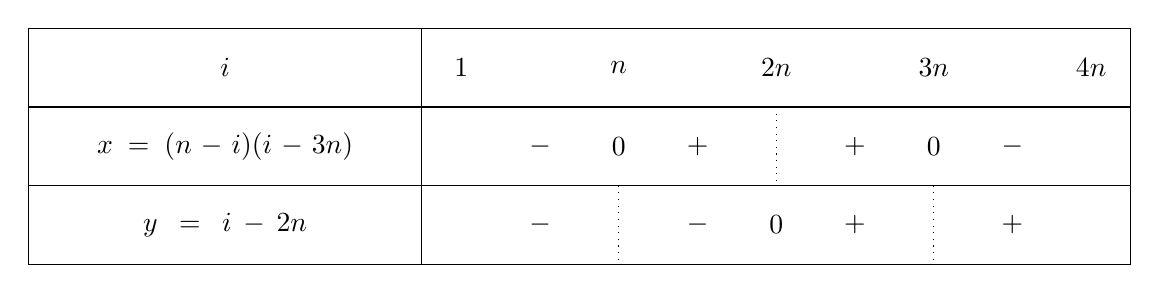
\begin{tikzpicture}
\tkzTabInit
[lgt=5,espcl=2] % tùy chọn
{$i$/1, $x=(n-i)(i-3n)$/1, $y=i-2n$/1} % cột đầu tiên
{$1$, $n$,$2n$,$3n$,$4n$} % hàng 1 cột 2
\tkzTabLine{,-,0,+,t,+,0,-,} % hàng 2 cột 2
\tkzTabLine{,-,t,-,0,+,t,+,} % hàng 3 cột 2
\end{tikzpicture}
\vspace{1em}\\
\textbf{Kết luận}
\begin{flalign*}
\displaystyle 
\text{Gán}(n)&=2+4\times4n+\sum_{i=1}^{4n}2\alpha_{i}+[3n-1-(2n+1)+1]\\&=17n+1+2\sum_{i=n+1}^{3n-1}\left\lceil\frac{(n-i)(i-3n)}{2}\right\rceil\\&\approx 17n+1+\frac{1}{3}n(4n^{2}-1)=\frac{4}{3}n^{3}+\frac{50}{3}n+1
\end{flalign*}
\begin{flalign*}
\displaystyle
\text{Sosánh}(n)&=4n+1+\sum_{i=1}^{4n}(\alpha_{i} +1)+4n+[3n-1-(n+1)+1]\\&=14n+\sum_{i=n+1}^{3n-1}\left\lceil\frac{(n-i)(i-3n)}{2}\right\rceil\\&\approx 14n+\frac{1}{3}n(4n^{2}-1)=\frac{41}{3}n+\frac{4}{3}n^{3}
\end{flalign*}
\section{Đếm số phép gán và so sánh}%Cau7
\begin{algorithm}[H]
    $i\gets 1$\Comment*[r]{2g}
    $count\gets 0$\;
    \While{$i\leq 4n$}{
        $x\gets (n-i)(i-3n)$\Comment*[r]{3g; 4n+1 ss}
        $y\gets i-2n$\;
        $j\gets 1$\;
        \While{$j\leq x$}{
            \If{$i\geq 2y$}{
                $count\gets count -2$\Comment*[r]{1g}
            }
            $j\gets j+1$\Comment*[r]{1g}
        }
        $i\gets i+1$\Comment*[r]{1g}
    }
\end{algorithm}
Gọi $\alpha_{i}$ là số lần lặp của vòng lặp \textbf{while} nhỏ với điều kiện $j \leq x$. \\
Vì $\alpha_{i}$ là số con $j$ mà $j$ chạy từ 1 $\rightarrow x$ với bước tăng là 1.\\
Do đó: 
\begin{flalign*}
\displaystyle\alpha_{i} \text{ là số phần tử của tập } \{1,2,3,\ldots,x\} &=x=(n-i)(i-3n)
\end{flalign*}
$\displaystyle\text{Với }\alpha_{i} \geq 1 \Leftrightarrow n+1 \leq i\leq 3n-1$.\\
Vậy:
\begin{gather*}
\alpha_{i}=\left\{\begin{array}{l}
    \displaystyle0,\quad  i \leq n \text{ hoặc } i\geq 3n\vspace{1em}\\
    \displaystyle(n-i)(i-3n), \quad n+1 \leq i\leq 3n-1
\end{array}\right.
\end{gather*}
Ta có bảng xét dấu:\\
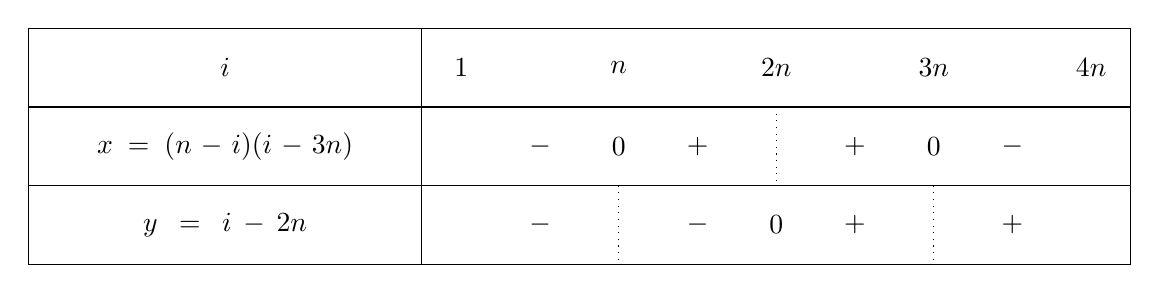
\begin{tikzpicture}
\tkzTabInit
[lgt=5,espcl=2] % tùy chọn
{$i$/1, $x=(n-i)(i-3n)$/1, $y=i-2n$/1} % cột đầu tiên
{$1$, $n$,$2n$,$3n$,$4n$} % hàng 1 cột 2
\tkzTabLine{,-,0,+,t,+,0,-,} % hàng 2 cột 2
\tkzTabLine{,-,t,-,0,+,t,+,} % hàng 3 cột 2
\end{tikzpicture}
Để câu lệnh $count\gets count -2$ được thực hiện $\Leftrightarrow i\leq 2y \Leftrightarrow i\leq 2(i-2n) \\\Leftrightarrow i\leq 4n \Rightarrow \text{ Câu lệnh luôn được thực hiện khi } \textbf{while } i\leq 4n \text{ thoả mãn}$.
\vspace{1em}\\
\textbf{Ta có}
\begin{flalign*}
\displaystyle 
\text{Gán}(n)&=2+4\times4n+\sum_{i=1}^{4n}2\alpha_{i}=2+16n+2\sum_{i=n+1}^{3n-1}(n-i)(i-3n)
\end{flalign*}
\begin{flalign*}
\displaystyle
\text{Sosánh}(n)&=4n+1+\sum_{i=1}^{4n}(\alpha_{i} +1)+\sum_{i=1}^{4n}\alpha_{i}\\&=8n+1+2\sum_{i=n+1}^{3n-1}(n-i)(i-3n)
\end{flalign*}
Xét:
\begin{multline*}
    \sum_{i=n+1}^{3n-1}(n-i)(i-3n)=\sum_{i=n+1}^{3n-1}(-3n^{2}+4ni-i^{2})\\=-3n^{2}\sum_{i=n+1}^{3n-1}1+4n\sum_{i=n+1}^{3n-1}i-\sum_{i=n+1}^{3n-1}i^{2}\\=-3n^{2}(2n-1)+4n\times 2n(2n-1)-\sum_{i=1}^{3n-1}i^{2}+\sum_{i=1}^{n}i^{2}\\=10n^{3}-5n^{2}-\frac{3n(3n-1)(6n-1)}{6}+\frac{n(n+1)(2n+1)}{6}=\frac{4n^{3}-n}{3}
\end{multline*}
\textbf{Kết luận}
\begin{flalign*}
\displaystyle 
\text{Gán}(n)&=2+16n+\frac{2}{3}(4n^{3}-n)=\frac{6+46n+8n^{3}}{3}
\end{flalign*}
\begin{flalign*}
\displaystyle
\text{Sosánh}(n)&=1+8n+\frac{2}{3}(4n^{3}-n)=\frac{3+22n+8n^{3}}{3}
\end{flalign*}
\section{Đếm số phép gán và so sánh} %Câu 8
\begin{algorithm}[H]
    $i\gets 1$\Comment*[r]{2g}
    $count\gets 0$\;
    \While{$i\leq 3n$}{
        $x\gets 2n-i$\Comment*[r]{3g; 3n+1 ss}
        $y\gets i-n$\;
        $j\gets 1$\;
        \While{$j\leq x$}{
            \If{$j\geq n$}{
                $count\gets count -1$\Comment*[r]{1g}
            }
            $j\gets j+1$\Comment*[r]{1g}
        }
        \If{$y>0$}{
            \If{$x>0$}{
                $count\gets count +1$\Comment*[r]{1g}
            }
        }
        $i\gets i+1$\Comment*[r]{1g}
    }
\end{algorithm}
Gọi $\alpha_{i}$ là số lần lặp của vòng lặp \textbf{while} nhỏ với điều kiện $j \leq x$. \\
Vì $\alpha_{i}$ là số con $j$ mà $j$ chạy từ 1 $\rightarrow x$ với bước tăng là 1.\\
Do đó: 
\begin{flalign*}
\displaystyle\alpha_{i} \text{ là số phần tử của tập } \{1,2,3,\ldots,x\} &=x=2n-i
\end{flalign*}
$\displaystyle\text{Với }\alpha_{i} \geq 1 \Leftrightarrow i\leq 2n-1$.
\vspace{1em}\\
Ta có bảng xét dấu:\\
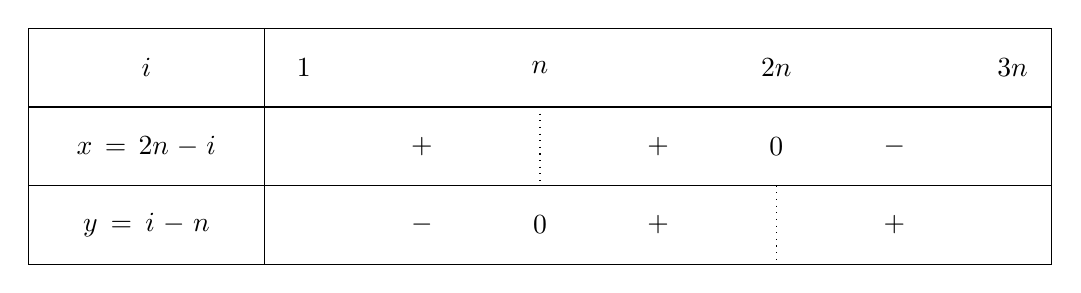
\begin{tikzpicture}
\tkzTabInit
[lgt=3,espcl=3] % tùy chọn
{$i$/1, $x=2n-i$/1, $y=i-n$/1} % cột đầu tiên
{$1$, $n$,$2n$,$3n$} % hàng 1 cột 2
\tkzTabLine{,+,t,+,0,-,} % hàng 2 cột 2
\tkzTabLine{,-,0,+,t,+,} % hàng 3 cột 2
\end{tikzpicture}
\vspace{1em}\\
Gọi $\beta_{i}$ là số lần câu lệnh \textbf{if} $j\geq n$ thoả mãn.\\
\begin{flalign*}
\beta_{i}=\text{ số phần tử của tập hợp }\{n,n+1,\ldots,x\}&=x-n+1\\&=2n-i-n+1=n-i+1
\end{flalign*}
Với $\beta_{i} \geq 1 \Leftrightarrow i\leq n$\\

Từ bảng xét dấu:
\begin{flalign*}
    x>0 \Leftrightarrow 1\leq i\leq 2n-1\\
    y>0 \Leftrightarrow n+1\leq i\leq 3n \\
    \left\{\begin{array}{l}
         x>0\\
         y>0
    \end{array}\Leftrightarrow n+1 \leq i\leq 2n-1\right.
\end{flalign*}
\textbf{Kết luận}
\begin{flalign*}
    \text{Gán}(n)&=2+4\times3n+\sum_{i=1}^{3n}\beta_{i}+\sum_{i=1}^{3n}\alpha_{i}+[2n-1-(n+1)+1]\\&=1+13n+\sum_{i=1}^{n}(n-i+1)+\sum_{i=1}^{2n-1}(2n-i)\\&=1+13n+(n+1)\sum_{i=1}^{n}1-\sum_{i=1}^{n}i+2n\sum_{i=1}^{2n-1}1-\sum_{i=1}^{2n-1}i\\&=1+13n+n(n+1)-\frac{n(n+1)}{2}+2n(2n-1)-\frac{2n(2n-1)}{2}\\&=\frac{5n^{2}+25n+2}{2}
\end{flalign*}
\begin{flalign*}
    \text{Sosánh}(n)&=3n+1+\sum_{i=1}^{3n}(\alpha_{i}+1)+\sum_{i=1}^{3n}\alpha_{i}+3n+[3n-(n+1)+1]\\&=1+8n+\sum_{i=1}^{3n}1+2\sum_{i=1}^{3n}\alpha_{i}\\&=1+11n+2\sum_{i=1}^{2n-1}(2n-i)\\&=1+11n+4n\sum_{i=1}^{2n-1}1-2\sum_{i=1}^{2n-1}i\\&=1+11n+4n(2n-1)-2\times\frac{2n(2n-1)}{2}=4n^{2}+9n+1
\end{flalign*}
\section{Đếm số phép gán và so sánh}%Câu 9
\begin{algorithm}[H]
    $i\gets 1$\Comment*[r]{2g}
    $res\gets 0$\;
    \While{$i\leq n$}{
        $j\gets 1$\Comment*[r]{2g; n+1 ss}
        $k\gets 1$\;
        \While{$j\leq i$}{
            $res\gets res+ij$\Comment*[r]{3g}
            $k\gets k+2$\;
            $j\gets j+k$\;
        }
        $i\gets i+1$\Comment*[r]{1g}
    }
\end{algorithm}
Gọi $\alpha_{i}$ là số lần lặp của vòng lặp \textbf{while} nhỏ với điều kiện $j \leq i$. \\
Vì $\alpha_{i}$ là số con $j$ mà $j$ chạy từ 1 $\rightarrow i$ với bước tăng là một cấp số cộng với số hạng đầu là $u_{1}=3$ và công bội $d=2$.\\
Do đó: 
\begin{flalign*}
\displaystyle\alpha_{i} \text{ là số phần tử của tập } \{1,4,9,\ldots,i\}=\text{số phần tử của tập } \{m\in \mathbb{N}^{\ast}\mid m^{2}\leq i\}
\end{flalign*}
Vậy:
\begin{flalign*}
    \alpha_{i} =\left\lfloor\sqrt{i}\right\rfloor
\end{flalign*}
\textbf{Kết luận}
\begin{flalign*}
    \text{Gán}(n)&=2+3n+\sum_{i=1}^{n}3\alpha_{i}=2+3n+3\sum_{i=1}^{n}\left\lfloor\sqrt{i}\right\rfloor\\&=2+3n+\frac{1}{2}\left\lfloor\sqrt{n}\right\rfloor\left(-2\left\lfloor\sqrt{n}\right\rfloor^{2}-3\left\lfloor\sqrt{n}\right\rfloor+6n+5\right)
\end{flalign*}
\begin{flalign*}
    \text{Sosánh}(n)&=n+1+\sum_{i=1}^{n}(\alpha_{i}+1)=2n+1+\sum_{i=1}^{n}\alpha_{i}\\&=2n+1+\sum_{i=1}^{n}\left\lfloor\sqrt{i}\right\rfloor\\&=2n+1+\frac{1}{6}\left\lfloor\sqrt{n}\right\rfloor\left(-2\left\lfloor\sqrt{n}\right\rfloor^{2}-3\left\lfloor\sqrt{n}\right\rfloor+6n+5\right)
\end{flalign*}
\section{Đếm số phép gán và so sánh} %Câu 10
\begin{algorithm}[H]
    $sum\gets 0$\Comment*[r]{3g}
    $i\gets 1$\;
    $idx\gets -1$\;
    \While{$i\leq n$}{
        $j\gets 1$\Comment*[r]{1g; n+1 ss}
        \While{$j\leq n$}{
            \If{$(i=j)$ AND $(i+j=n+1)$}{
                $idx\gets i$\;
            }
            $sum\gets sum+a[i][j]$\Comment*[r]{2g; n+1 ss}
            $j\gets j+1$\;
        }
        $i\gets i+1$\Comment*[r]{1g}
    }
    \If{$idx\neq -1$}{
        $sum\gets sum -a[idx][idx]$\;
    }
\end{algorithm}
Để gán $idx\gets i:\left\{\begin{array}{c}
     i=j  \\
     i+j=n+1 
\end{array}\right.\Leftrightarrow 2i=n+1\Leftrightarrow n$ lẻ\\
\textit{Nhận xét:}
\begin{enumerate}[label={TH \arabic*:}]
    \item $n$ lẻ $\rightarrow$ tồn tại duy nhất 1 trường hợp thoả mãn điều kiện để $idx \gets i$, khi đó:
        \begin{flalign*}
            &\text{Gán}(n)=3+2n+(1+2n^{2})+1=2n^{2}+2n+5\\
            &\text{Sosánh}(n)=n+1+n(n+1)+2n^{2}+1=3n^{2}+2n+2
        \end{flalign*}
    \item $n$ chẵn $\rightarrow$ không tồn tại trường hợp thoả mãn điều kiện $\Rightarrow idx\gets -1$, khi đó: 
        \begin{flalign*}
            &\text{Gán}(n)=3+2n+2n^{2}\\
            &\text{Sosánh}(n)=n+1+n(n+1)+2n^{2}+1=3n^{2}+2n+2
        \end{flalign*}
\end{enumerate}
\textbf{Kết luận}
\begin{flalign*}
    \text{Gán}(n)=\left\{\begin{array}{l}
         2n^{2}+2n+5,\quad n \text{ lẻ}  \\
         2n^{2}+2n+3,\quad n \text{ chẵn}
    \end{array}\right.
\end{flalign*}
\begin{flalign*}
    \text{Sosánh}(n)=3n^{2}+2n+2
\end{flalign*}
\section{Đếm và kiểm tra số phép gán, so sánh} %Câu 11
\begin{algorithm}[H]
    $i\gets 1$\;
    $ret\gets 0$\;
    $s\gets 0$\;
    \While{$i\leq n$}{
        $j\gets 1$\;
        $s\gets s+1/i$; \tcp{số thực}
        \While{$j\leq s$}{
            $ret\gets ret+ij$\;
            $j\gets j+1$\;
        }
        $i\gets i+1$\;
    }
\end{algorithm}
\subsection{Kỹ thuật toán sơ cấp}
Gọi $\alpha_{i}$ là số lần lặp của vòng lặp \textbf{while} nhỏ với điều kiện $j \leq s$. \\
Vì $\alpha_{i}$ là số con $j$ mà $j$ chạy từ 1 $\rightarrow s$ với bước tăng 1.\\
Mặt khác:
\begin{flalign*}
    s \text{ nhận các giá trị } \left\{1, 1+\frac{1}{2},\ldots, 1+\frac{1}{2}+\frac{1}{3}+\ldots+\frac{1}{i}\right\}
\end{flalign*}
Do đó: 
\begin{flalign*}
\displaystyle\alpha_{i} \text{ là số phần tử của tập } \{1,2,3,\ldots,s\}=s=\left\lfloor\sum_{x=1}^{i}\frac{1}{x}\right\rfloor
\end{flalign*}
\textbf{Kết luận}
\begin{flalign}
\begin{split}
    \text{Gán}(n)&=3+3n+\sum_{i=1}^{n}2\alpha_{i}\\&=3+3n+2\sum_{i=1}^{n}\left\lfloor\sum_{x=1}^{i}\frac{1}{x}\right\rfloor
\end{split}
    \\&\approx 3+3n+2\sum_{i=1}^{n}\left\lfloor\ln i+\gamma\right\rfloor\quad (\gamma \approx 0.5772)
\end{flalign}
\begin{flalign}
    \text{Sosánh}(n)&=n+1+\sum_{i=1}^{n}(\alpha_{i}+1)=2n+1+\sum_{i=1}^{n}\left\lfloor\sum_{x=1}^{i}\frac{1}{x}\right\rfloor\\&\approx 2n+1+\sum_{i=1}^{n}\left\lfloor\ln i+\gamma\right\rfloor\quad (\gamma \approx 0.5772) 
\end{flalign}
\subsection{Kiểm tra bằng chương trình \texttt{C++}}
\begin{lstlisting}
// The function counts the number of assignments and comparisons performed in the process based on n.
// The function takes three parameters: n (the upper limit), Assign (a vector to store the assignment counts), Compare (a vector to store the comparison counts).
void Function(int n, vector<int>& Assign, vector<int>& Compare){
    float i = 1, ret = 0, s = 0, j;
    int count_assign = 3, count_compare = 0;
    // Increment compare counter
    count_compare++;
    // Loop from 1 to n
    while (i <= n){ 
        count_compare++;
        // Initialize j
        j = 1; 
        count_assign++;
        s = s + (1 / i);
        count_assign++;
        count_compare++;
        // Loop from 1 to s
        while (j <= s){ 
            count_compare++;
            ret = ret + i * j;
            count_assign++;
            // Increment j
            j = j + 1; 
            count_assign++;
        }
        // Increment i
        i = i + 1; 
        count_assign++;
    }
    // Store assign counter in vector
    Assign.push_back(count_assign);
    // Store compare counter in vector
    Compare.push_back(count_compare); 
}

int main(){
    int n;
    vector<int> Assign;
    vector<int> Compare;
    cout << "n\t\t";
    // Print values of n from 1 to 20
    for (int i = 1; i <= 20; i++) cout << i << "\t";
    // Call function for each value of n
    for (n = 1; n <= 20; n++) Function(n, Assign, Compare); 
    cout << "\nGan(n)      ";
    // Print assign values for each n
    for (int i = 0; i < 20; i++) cout << Assign[i] << "\t"; 
    cout << "\nSosanh(n)   ";
    // Print compare values for each n
    for (int i = 0; i < 20; i++) cout << Compare[i] << "\t"; 
    return 0;
}
\end{lstlisting}
\begin{center}
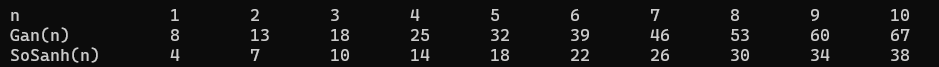
\includegraphics[width=1\textwidth]{img/terminal11a.png}
\captionof{figure}{Kết quả chạy chương trình với $n \in [1,10]$}   
\end{center}
\begin{center}
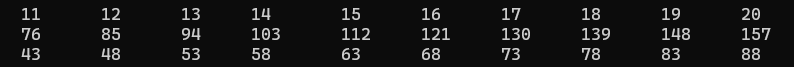
\includegraphics[width=1\textwidth]{img/terminal11b.png}
\captionof{figure}{Kết quả chạy chương trình với $n \in [11,20]$}   
\end{center}

\tikzset{ 
    table/.style={
        matrix of nodes,
        row sep=-\pgflinewidth,
        column sep=-\pgflinewidth,
        nodes={
            rectangle,
            draw=black,
            align=center
        },
        minimum height=1.5em,
        text depth=0.5ex,
        text height=2ex,
        nodes in empty cells,
%%
        every even row/.style={
            nodes={fill=gray!20}
        },
        column 1/.style={
            nodes={text width=2em}
        },
        row 1/.style={
            nodes={
            }
        }
    }
}
\newpage
\begin{center}
\captionof{table}{Bảng thống kê so sánh kết quả giữa công thức và chương trình}
\begin{tikzpicture}
\matrix (first) [table,text width=6em]
{
n & Gán$(n)=(1)$    & Code & SS$(n)=(3)$ & Code \\
1   & 8 & 8 & 4 & 4  \\
2   & 13 & 13 & 7 & 7  \\
3   & 18 & 18 & 10 & 10  \\
4   & 25 & 25 & 14 & 14  \\
5   & 32 & 32 & 18 & 18  \\
6   & 39 & 39 & 22 & 22  \\
7   & 46 & 46 & 26 & 26  \\
8   & 53 & 53 & 30 & 30  \\
9   & 60 & 60 & 34 & 34  \\
10   & 67 & 67 & 38 & 38  \\
11   & 76 & 76 & 43 & 43  \\
12   & 85 & 85 & 48 & 48  \\
13   & 94 & 94 & 53 & 53  \\
14   & 103 & 103 & 58 & 58  \\
15   & 112 & 112 & 63 & 63  \\
16   & 121 & 121 & 68 & 68  \\
17   & 130 & 130 & 73 & 73  \\
18   & 139 & 139 & 78 & 78  \\
19   & 148 & 148 & 83 & 83  \\
20   & 157 & 157 & 88 & 88  \\
};
\end{tikzpicture}
\end{center}
\section{Đếm và kiểm tra số phép gán, so sánh}
\begin{algorithm}[H]
    $i\gets 1$\;
    $res\gets 0$\;
    \While{$i\leq n$}{
        $j\gets 1$\;
        \While{$j\leq i$}{
            $res\gets res+ij$\;
            $j\gets j+1$\;
        }
        $i\gets i+5$\;
    }
\end{algorithm}
\subsection{Kỹ thuật toán sơ cấp}
Đặt $\displaystyle i=1+5k \Rightarrow 1\leq 1+5k \leq n \Rightarrow 0\leq k\leq \left\lfloor\frac{n-1}{5}\right\rfloor$\\
Khi đó số lần lặp vòng \textbf{while} ngoài chính là số giá trị $k$ thoả mãn điều kiện trên.\\
$\Rightarrow$ số lần lặp vòng while ngoài $\displaystyle=\left\lfloor\frac{n-1}{5}\right\rfloor + 1$.
Gọi $\alpha_{i}$ là số lần lặp của vòng lặp \textbf{while} nhỏ với điều kiện $j \leq i$. \\
Vì $\alpha_{i}$ là số con $j$ mà $j$ chạy từ 1 $\rightarrow i$ với bước tăng 1.\\
Do đó: 
\begin{flalign*}
\displaystyle\alpha_{i} \text{ là số phần tử của tập } \{1,2,3,\ldots,i\}=1+5k
\end{flalign*}
\textbf{Kết luận}
\begin{flalign}
\begin{split}
    \displaystyle
    \text{Gán}(n)&=2+2\left(\left\lfloor\frac{n-1}{5}\right\rfloor + 1\right)+\sum_{k=0}^{\left\lfloor\frac{n-1}{5}\right\rfloor}2\alpha_{i}\\&=4+2\left\lfloor\frac{n-1}{5}\right\rfloor+2\sum_{k=0}^{\left\lfloor\frac{n-1}{5}\right\rfloor}(1+5k)\\&=4+2\left\lfloor\frac{n-1}{5}\right\rfloor+2\sum_{k=0}^{\left\lfloor\frac{n-1}{5}\right\rfloor}1+10\sum_{k=0}^{\left\lfloor\frac{n-1}{5}\right\rfloor}k\\&=4+2\left\lfloor\frac{n-1}{5}\right\rfloor+2\left(\left\lfloor\frac{n-1}{5}\right\rfloor+1\right)+5\left\lfloor\frac{n-1}{5}\right\rfloor\left(\left\lfloor\frac{n-1}{5}\right\rfloor+1\right)\\&=6+9\left\lfloor\frac{n-1}{5}\right\rfloor+5\left\lfloor\frac{n-1}{5}\right\rfloor^{2}
\end{split}
\end{flalign}
\begin{flalign}
\begin{split}
    \displaystyle
    \text{Sosánh}(n)&=\left(\left\lfloor\frac{n-1}{5}\right\rfloor+1\right)+1+\sum_{k=0}^{\left\lfloor\frac{n-1}{5}\right\rfloor}(\alpha_{i}+1)\\&=2+\left\lfloor\frac{n-1}{5}\right\rfloor+\sum_{k=0}^{\left\lfloor\frac{n-1}{5}\right\rfloor}1+\sum_{k=0}^{\left\lfloor\frac{n-1}{5}\right\rfloor}\alpha_{i}\\&=2+\left\lfloor\frac{n-1}{5}\right\rfloor+\left\lfloor\frac{n-1}{5}\right\rfloor+1+\sum_{k=0}^{\left\lfloor\frac{n-1}{5}\right\rfloor}(1+5k)\\&=3+2\left\lfloor\frac{n-1}{5}\right\rfloor+\sum_{k=0}^{\left\lfloor\frac{n-1}{5}\right\rfloor}1+5\sum_{k=0}^{\left\lfloor\frac{n-1}{5}\right\rfloor}k\\&=4+\frac{11}{2}\left\lfloor\frac{n-1}{5}\right\rfloor+\frac{5}{2}\left\lfloor\frac{n-1}{5}\right\rfloor^{2}
\end{split}
\end{flalign}
\subsection{Kiểm tra bằng chương trình \texttt{C++}}
\begin{lstlisting}
// The function counts the number of assignments and comparisons performed in the process based on n.
// The function takes three parameters: n (the upper limit), Assign (a vector to store the assignment counts), Compare (a vector to store the comparison counts)
void Function(int n, vector<int> &Assign, vector<int> &Compare){
    // Initialize i to 1 
    int i = 1, res = 0; 
    // Initialize count_assign and count_compare to 2 and 1 respectively
    int count_assign = 2, count_compare = 1;
    // Loop from i to n with a step of 5
    while (i <= n){
        // Initialize j to 1
        int j = 1; 
        // Increment count_assign by one
        count_assign++;
        // Increment count_compare by one
        count_compare++;
        // Loop from j to i with a step of one
        while (j <= i){ 
            res = res + i * j;
            // Increment j by one
            j = j + 1;
            // Increment count_assign by two
            count_assign += 2;
            // Increment count_compare by one
            count_compare++; 
        }
        // Increment i by five
        i = i + 5;
        // Increment count_assign and count_compare by one
        count_assign++;  
        count_compare++;
    }
    // Append the final value of count_assign to Assign vector 
    Assign.push_back(count_assign);
    // Append the final value of count_compare to Compare vector
    Compare.push_back(count_compare);  
}

int main(){
    // Declare an integer variable n
    int n;
    // Declare a vector variable Assign
    vector<int> Assign;
    // Declare a vector variable Compare
    vector<int> Compare;  
    cout << "n\t\t";
    // Print values of n from 1 to 20 separated by tabs
    for (int i = 1; i <= 20; i++) cout << i << "\t";
    // Call Function for each value of n from 1 to 20 and pass Assign and Compare vectors as arguments
    for (n = 1; n <= 20; n++) Function(n, Assign, Compare);  
    cout << "\nGan(n)      ";
    // Print assign values for each n separated by tabs 
    for (int i = 0; i < 20; i++) cout << Assign[i] << "\t"; 
    cout << "\nSosanh(n)   ";
    // Print compare values for each n separated by tabs
    for (int i = 0; i < 20; i++) cout << Compare[i] << "\t"; 
    return 0;
}
\end{lstlisting}
\begin{center}
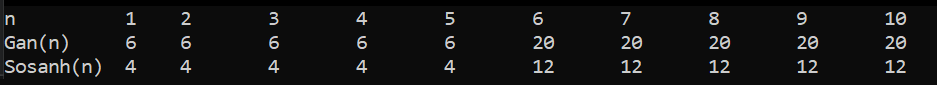
\includegraphics[width=1\textwidth]{img/terminal12a.png}
\captionof{figure}{Kết quả chạy chương trình với $n \in [1,10]$}   
\end{center}
\begin{center}
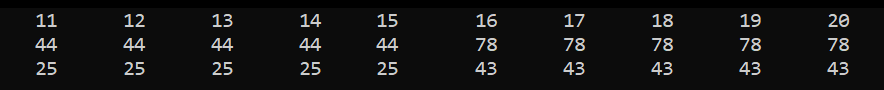
\includegraphics[width=1\textwidth]{img/terminal12b.png}
\captionof{figure}{Kết quả chạy chương trình với $n \in [11,20]$}   
\end{center}
\newpage
\begin{center}
\captionof{table}{Bảng thống kê so sánh kết quả giữa công thức và chương trình}
\begin{tikzpicture}
\matrix (first) [table,text width=6em]
{
n & Gán$(n)=(5)$    & Code & SS$(n)=(6)$ & Code \\
1   & 6 & 6 & 4 & 4  \\
2   & 6 & 6 & 4 & 4  \\
3   & 6 & 6 & 4 & 4  \\
4   & 6 & 6 & 4 & 4  \\
5   & 6 & 6 & 4 & 4  \\
6   & 20 & 20 & 12 & 12  \\
7   & 20 & 20 & 12 & 12  \\
8   & 20 & 20 & 12 & 12  \\
9   & 20 & 20 & 12 & 12  \\
10   & 20 & 20 & 12 & 12  \\
11   & 44 & 44 & 25 & 25  \\
12   & 44 & 44 & 25 & 25  \\
13   & 44 & 44 & 25 & 25  \\
14   & 44 & 44 & 25 & 25  \\
15   & 44 & 44 & 25 & 25  \\
16   & 78 & 78 & 43 & 43  \\
17   & 78 & 78 & 43 & 43  \\
18   & 78 & 78 & 43 & 43  \\
19   & 78 & 78 & 43 & 43  \\
20   & 78 & 78 & 43 & 43  \\
};
\end{tikzpicture}
\end{center}
\section{Đếm và kiểm tra số phép gán, so sánh} %câu 13
\begin{algorithm}[H]
    $sum\gets 0$\;
    $i\gets n$\;
    \While{$i>0$}{
        $j\gets i$\;
        \While{$j>0$}{
            $sum\gets sum+1$\;
            $j\gets j-1$\;
        }
        $i\gets i \div 2$\;
    }
\end{algorithm}
\subsection{Kỹ thuật toán sơ cấp}
Đặt $\displaystyle i=\frac{n}{2^{k}} \Rightarrow 0 < i \leq n \Leftrightarrow 1 \leq \frac{n}{2^{k}}\leq n \Rightarrow 0 \leq k\leq \left\lfloor\log_{2}n\right\rfloor$\\
Khi đó số lần lặp vòng \textbf{while} ngoài chính là số giá trị $k$ thoả mãn điều kiện trên.\\
$\Rightarrow$ số lần lặp vòng while ngoài $\displaystyle=\left\lfloor\log_{2}n\right\rfloor + 1$.\\
Gọi $\alpha_{i}$ là số lần lặp của vòng lặp \textbf{while} nhỏ với điều kiện $j \geq 0$. \\
Vì $\alpha_{i}$ là số con $j$ mà $j$ chạy từ i $\rightarrow 1$ với bước giảm 1.\\
Do đó: 
\begin{flalign*}
\displaystyle\alpha_{i} \text{ là số phần tử của tập } \{i,i-1,i-2,\ldots,1\}=i=\left\lfloor\frac{n}{2^{k}}\right\rfloor
\end{flalign*}
\textbf{Kết luận}
\begin{flalign}
    \begin{split}
        \text{Gán}(n)&=2+2\left(\left\lfloor\log_{2}n\right\rfloor+1\right)+\sum_{k=0}^{\left\lfloor\log_{2}n\right\rfloor}2\alpha_{i}\\&=4+2\left\lfloor\log_{2}n\right\rfloor+2\sum_{k=0}^{\left\lfloor\log_{2}n\right\rfloor}\alpha_{i}\\&=4+2\left\lfloor\log_{2}n\right\rfloor+2\sum_{k=0}^{\left\lfloor\log_{2}n\right\rfloor}\left\lfloor\frac{n}{2^{k}}\right\rfloor
    \end{split}
        \\&\approx 4+2\left\lfloor\log_{2}n\right\rfloor+4n-2= 2+4n+2\left\lfloor\log_{2}n\right\rfloor  
\end{flalign}
\begin{flalign}
    \begin{split}
        \text{Sosánh}(n)&=\left(\left\lfloor\log_{2}n\right\rfloor+1\right)+1+\sum_{k=0}^{\left\lfloor\log_{2}n\right\rfloor}(\alpha_{i}+1)\\&=2+\left\lfloor\log_{2}n\right\rfloor+\sum_{k=0}^{\left\lfloor\log_{2}n\right\rfloor}\alpha_{i}+\sum_{k=0}^{\left\lfloor\log_{2}n\right\rfloor}1\\&=2+\left\lfloor\log_{2}n\right\rfloor+\left\lfloor\log_{2}n\right\rfloor+1+\sum_{k=0}^{\left\lfloor\log_{2}n\right\rfloor}\left\lfloor\frac{n}{2^{k}}\right\rfloor\\&=3+2\left\lfloor\log_{2}n\right\rfloor+\sum_{k=0}^{\left\lfloor\log_{2}n\right\rfloor}\left\lfloor\frac{n}{2^{k}}\right\rfloor
    \end{split}
        \\&\approx 3+2\left\lfloor\log_{2}n\right\rfloor+2n-1= 2+2n+2\left\lfloor\log_{2}n\right\rfloor
\end{flalign}
\subsection{Kiểm tra bằng chương trình \texttt{C++}}
\begin{lstlisting}
// The function counts the number of assignments and comparisons performed in the process based on n.
// The function takes three parameters: n (the upper limit), Assign (a vector to store the assignment counts), Compare (a vector to store the comparison counts)
void Function(int n, vector<int> &Assign, vector<int> &Compare){
    int sum = 0;
    // Initialize i to n
    int i = n;
    // Initialize count_assign and count_compare to 2 and 1 respectively
    int count_assign = 2, count_compare = 1;
    // Loop from i to zero with a step of dividing by two
    while (i > 0){
        // Initialize j to i
        int j = i;
        count_assign++;
        count_compare++;
        // Loop from j to zero with a step of subtracting one 
        while (j > 0){
            sum = sum + 1;
            j = j - 1;
            count_assign += 2;
            count_compare += 1;
        }
        i = i / 2;
        count_assign++;
        count_compare++;
    }
    // Append the final value of count_assign to Assign vector 
    Assign.push_back(count_assign);
    // Append the final value of count_compare to Compare vector
    Compare.push_back(count_compare);  
}

int main(){
    // Declare an integer variable n
    int n;
    // Declare a vector variable Assign
    vector<int> Assign;
    // Declare a vector variable Compare
    vector<int> Compare;  
    cout << "n\t\t";
    // Print values of n from 1 to 20 separated by tabs
    for (int i = 1; i <= 20; i++) cout << i << "\t";
    // Call Function for each value of n from 1 to 20 and pass Assign and Compare vectors as arguments
    for (n = 1; n <= 20; n++) Function(n, Assign, Compare);  
    cout << "\nGan(n)      ";
    // Print assign values for each n separated by tabs 
    for (int i = 0; i < 20; i++) cout << Assign[i] << "\t"; 
    cout << "\nSosanh(n)   ";
    // Print compare values for each n separated by tabs
    for (int i = 0; i < 20; i++) cout << Compare[i] << "\t"; 
    return 0;
}
\end{lstlisting}
\begin{center}
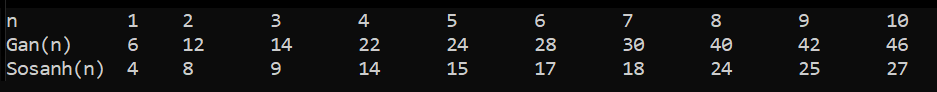
\includegraphics[width=1\textwidth]{img/terminal13a.png}
\captionof{figure}{Kết quả chạy chương trình với $n \in [1,10]$}   
\end{center}
\begin{center}
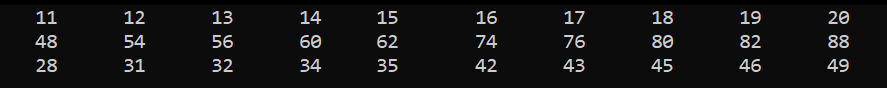
\includegraphics[width=1\textwidth]{img/terminal13b.png}
\captionof{figure}{Kết quả chạy chương trình với $n \in [11,20]$}   
\end{center}
\begin{center}
\captionof{table}{Bảng thống kê so sánh kết quả giữa công thức và chương trình}
\begin{tikzpicture}
\matrix (first) [table,text width=6em]
{
n & Gán$(n)=(7)$    & Code & SS$(n)=(9)$ & Code \\
1   & 6 & 6 & 4 & 4  \\
2   & 12 & 12 & 8 & 8  \\
3   & 14 & 14 & 9 & 9  \\
4   & 22 & 22 & 14 & 14  \\
5   & 24 & 24 & 15 & 15  \\
6   & 28 & 28 & 17 & 17  \\
7   & 30 & 30 & 18 & 18  \\
8   & 40 & 40 & 24 & 24  \\
9   & 42 & 42 & 25 & 25  \\
10   & 46 & 46 & 27 & 27  \\
11   & 48 & 48 & 28 & 28  \\
12   & 54 & 54 & 31 & 31  \\
13   & 56 & 56 & 32 & 32  \\
14   & 60 & 60 & 34 & 34  \\
15   & 62 & 62 & 35 & 35  \\
16   & 74 & 74 & 42 & 42  \\
17   & 76 & 76 & 43 & 43  \\
18   & 80 & 80 & 45 & 45  \\
19   & 82 & 82 & 46 & 46  \\
20   & 88 & 88 & 49 & 49  \\
};
\end{tikzpicture}
\end{center}
\end{document}
